\documentclass{beamer}
\usetheme{Montpellier}
\usecolortheme{dolphin}

%\usepackage{graphicx} %For jpg figure inclusion
%\usepackage{times} %For typeface
%\usepackage{epsfig}
\usepackage{color} %For Comments
\usepackage{beamerthemeshadow} %Paul and Lemmon put this in, take out if you want
%\usepackage[all]{xy}
%\usepackage{float}
%\usepackage{subfigure} 
%\usepackage{hyperref}
%\usepackage{url}
%\usepackage{parskip}
%\usepackage{multirow}

%% Elena's favorite green (thanks, Fernando!)
\definecolor{ForestGreen}{RGB}{34,139,34}
\definecolor{BlueViolet}{RGB}{138,43,226}
\definecolor{Coquelicot}{RGB}{255, 56, 0}
\definecolor{Teal}{RGB}{2,132,130}
% Uncomment this if you want to show work-in-progress comments
\newcommand{\comment}[1]{{\bf \tt  {#1}}}
% Uncomment this if you don't want to show comments
%\newcommand{\comment}[1]{}
\newcommand{\emcomment}[1]{\textcolor{ForestGreen}{\comment{Elena: {#1}}}}
\newcommand{\todo}[1]{\textcolor{blue}{\comment{To Do: {#1}}}}
\newcommand{\pscomment}[1]{\textcolor{Coquelicot}{\comment{Paul: {#1}}}}
\newcommand{\mmcomment}[1]{\textcolor{magenta}{\comment{Max: {#1}}}}
\newcommand{\escomment}[1]{\textcolor{BlueViolet}{\comment{Emma: {#1}}}}
\newcommand{\alcomment}[1]{\textcolor{red}{\comment{Lemmon: {#1}}}}
\newcommand{\hfcomment}[1]{\textcolor{Teal}{\comment{Henry: {#1}}}}
%%%%%%%%%%%%%%%%%%%%%%%%%%%%%%%%%%%%%%%%%%

\begin{document}
\title{Developing Beginner-Friendly User Interactions for the Clojure Programming Language}
\date{April 11, 2015}

\begin{frame}
\frametitle{Developing Beginner-Friendly User Interactions for the Clojure Programming Language}
{\centering
\noindent
Henry Fellows, Aaron Lemmon, Max Magnuson, \par
Emma Sax, Paul Schliep, and Elena Machkasova \par

{\it 
Midwest Instruction and Computing Symposium\par
April 11, 2015\par}
}
\end{frame}
%frame

\begin{frame}
\frametitle{Table of contents}
\tableofcontents  
\end{frame}

\section{Overview of Clojure}

\begin{frame}
\frametitle{Intro to Clojure and Clojure attributes}
	\begin{itemize}
  	 \item Developed in 2007 by Rich Hickey
  	 \item Dynamic
  	 \item Functional
  	 \item A Lisp language
  	 \item Runs on the Java Virtual Machine (JVM)
  	 \item Clojure's read-eval-print-loop (REPL)
  	 \item Focus on immutable data types
	 \end{itemize}
\end{frame}

\begin{frame}[fragile]
\frametitle{Prefix Notation}
	\begin{itemize}
  	 \item Clojure uses prefix notation
  	 \begin{itemize}
  	 	\item parentheses
  	 	\item parameters
  	 %\end{itemize}
  	 \begin{verbatim}
		(<function-name> <argument 1> <argument 2>)
	 \end{verbatim}
	 \end{itemize}
	\end{itemize}
	\begin{itemize}
  	 	\item A simple example
  	 	\begin{itemize}
  	 	 \item \texttt{+} is a built-in function, not an operation
  	 	%\end{itemize}
  	 	\begin{verbatim}		
		(+ 5 5)
		-> 10
	    \end{verbatim}
	    \end{itemize}
  	 \end{itemize}
\end{frame}

\begin{frame}[fragile]
\frametitle{Defining Functions and Variables}
	\begin{itemize}
  	 \item \texttt{def} can be used to define variables
  	 \begin{verbatim}
		(def mystring "Hello World")
		mystring
		-> "Hello World"
	\end{verbatim}
	\end{itemize}
	\begin{itemize}
  	 \item \texttt{defn} can be used to define functions
  	 \begin{verbatim}
		(defn increment-number [number] (+ number 1))
		(increment-number 2)
		-> 3
	\end{verbatim}
	\end{itemize}
\end{frame}

\begin{frame}[fragile]
\frametitle{Anonymous Functions}
	\begin{itemize}
  	 \item Anonymous functions are a way to implement a function on the fly, and use it only once\
  	 \item A simple example
  	 \begin{itemize}
  	 	\item \texttt{map} takes a function and a collection as arguments, and applies the function to the entire collection
  	 %\end{itemize}
  	 	\begin{verbatim}
		(map (fn [number] (+ number 1)) [0 1 2 3])
		-> (1 2 3 4)
	\end{verbatim}
	\end{itemize}
	\end{itemize}
\end{frame}

\begin{frame}[fragile]
\frametitle{Collections}
    \begin{itemize}
     \item All collections can contain any number of values of any data type
	 \begin{itemize}
	  \item Lists
	  \begin{verbatim}
	   (1 2 "foo" :a 9 "bar")
	  \end{verbatim}
  	  \item Vectors
  	  \begin{verbatim}
	   [1 2 "foo" :a 9 "bar"]
	  \end{verbatim}
  	  \item Sets
  	  \begin{verbatim}
	   #{1 2 "foo" :a 9 "bar"}
	  \end{verbatim}
  	  \item Hashmaps
  	  \begin{itemize}
  	 	 \item key-value pairs
  	  \end{itemize}
  	  %\end{itemize}
  	  \begin{verbatim}
	    	{:a 1, :b 2, :c 3}
	  \end{verbatim}
	 \end{itemize}
    \end{itemize}
\end{frame}

\begin{frame}[fragile]
\frametitle{Laziness}
	\begin{itemize}
  	  \item The evaluation of an expression is postponed until the return value is needed
  	  \begin{itemize}
  	    \item Fibonacci sequence
  	  \end{itemize}
  	  \item A simple example
  	  \begin{itemize}
  	    \item \texttt{take} takes the first $n$ elements of a collection
  	    \item \texttt{range} returns an infinite sequence of non-negative integers beginning at 0
  	  \end{itemize}
  	  \begin{verbatim}
  	 	(take 10 (range))
  	 	-> (0 1 2 3 4 5 6 7 8 9)
  	  \end{verbatim}
  	  \item A common example
  	  \begin{verbatim}
  	 	(if (< number 10) (+ number 1) (- number 1))
  	  \end{verbatim}
   \end{itemize}
\end{frame}

\section{Error Messages}

\begin{frame}
\frametitle{Clojure error messages: background}
	\begin{itemize}
  		\item Error messages should be:
  		\begin{itemize}
  	 		\item helpful for debugging
  	 		\item easy to understand
  	 		\item approachable
  		\end{itemize}
  		\item Clojure error messages are confusing
	 \end{itemize}
	 
\end{frame}

\begin{frame}[fragile]
\frametitle{Clojure error messages: example}

\begin{verbatim}
Exception in thread "main" java.lang.RuntimeException: EOF while reading, starting at line 3, compiling:(compilation_errors/eof.clj:4:1)
	at clojure.lang.Compiler.load(Compiler.java:7137)
	at clojure.lang.RT.loadResourceScript(RT.java:370)
	at clojure.lang.RT.loadResourceScript(RT.java:361)
	at clojure.lang.RT.load(RT.java:440)
	at clojure.lang.RT.load(RT.java:411)
	at clojure.core$load$fn__5066.invoke(core.clj:5641)
	at clojure.core$load.doInvoke(core.clj:5640)
	at clojure.lang.RestFn.invoke(RestFn.java:408)
	at clojure.core$load_one.invoke(core.clj:5446)
	at clojure.core$load_lib$fn__5015.invoke(core.clj:5486)
	at clojure.core$load_lib.doInvoke(core.clj:5485)
	at clojure.lang.RestFn.applyTo(RestFn.java:142)
	at clojure.core$apply.invoke(core.clj:626)
	at clojure.core$load_libs.doInvoke(core.clj:5524)
	at clojure.lang.RestFn.applyTo(RestFn.java:137)
	at clojure.core$apply.invoke(core.clj:626)
	at clojure.core$require.doInvoke(core.clj:5607)
\end{verbatim}

\end{frame}

\begin{frame}
\frametitle{Error message transformations: try/catch}
	\begin{itemize}
  	 \item wrap user's code in try/catch block
  	 \item capture the error message and check it against numerous regular expressions
  	 \item once matched, replaced with improved message
	 \end{itemize}
	 Pros and Cons:
	 \begin{itemize}
	 \item able to handle both runtime and compilation exceptions
	 \item usually cannot recover argument values
	 \item additional complexity with REPL and lazy sequences
	 \end{itemize}
\end{frame}

\begin{frame}
\frametitle{Error message transformations: function substitution}
	\begin{itemize}
  	 \item override built-in functions with identical ones that include type checking
  	 \item potential errors can be detected with the type checks and a custom error message may be shown
	 \end{itemize}
	 Pros and Cons:
	 \begin{itemize}
	 \item unable to handle compilation exceptions
	 \item able to recover argument values and use them for a more meaningful message
	 \item can not handle student made functions
	 \item impractical to redefine all existing functions
	 \end{itemize}
\end{frame}

\begin{frame}[fragile]
\frametitle{User scenarios: example}
	Erroneous code fragment:
	\begin{verbatim}
	(defn square-this (* input input))
	
	-> IllegalArgumentException Parameter declaration
	* should be a vector 
	clojure.core/assert-valid-fdecl (core.clj:6842)
	\end{verbatim}
	
	Corrected Code:
	\begin{verbatim}
	(defn square-this [input] (* input input))
	\end{verbatim}
\end{frame}

\begin{frame}
\frametitle{User scenarios: explanation}
	\begin{itemize}
  	 \item Fill in things here......
	 \end{itemize}
\end{frame}

\begin{frame}
\frametitle{Hints: How they are helpful}
	\begin{itemize}
  	 \item Fill in things here......
	 \end{itemize}
\end{frame}

\begin{frame}
\frametitle{Hints: example}
	\begin{itemize}
  	 \item Fill in things here......
	 \end{itemize}
\end{frame}

\begin{frame}
\frametitle{Hints: future work}
	\begin{itemize}
  	 \item Fill in things here......
	 \end{itemize}
\end{frame}
% Henry & Max
\section{Technical Setup}
\begin{frame}
\frametitle{Setup}
	\begin{itemize}
		\item IDE
		\begin{itemize}
			\item LightTable
			\item Nightcode
		\end{itemize}
		\item Leiningen
		\begin{itemize}
			\item project manager
			\item popular in Clojure community
		\end{itemize}
	\end{itemize}
\end{frame}

\begin{frame}[fragile]
\frametitle{Current Workflow Diagram}
\begin{figure}[h]
 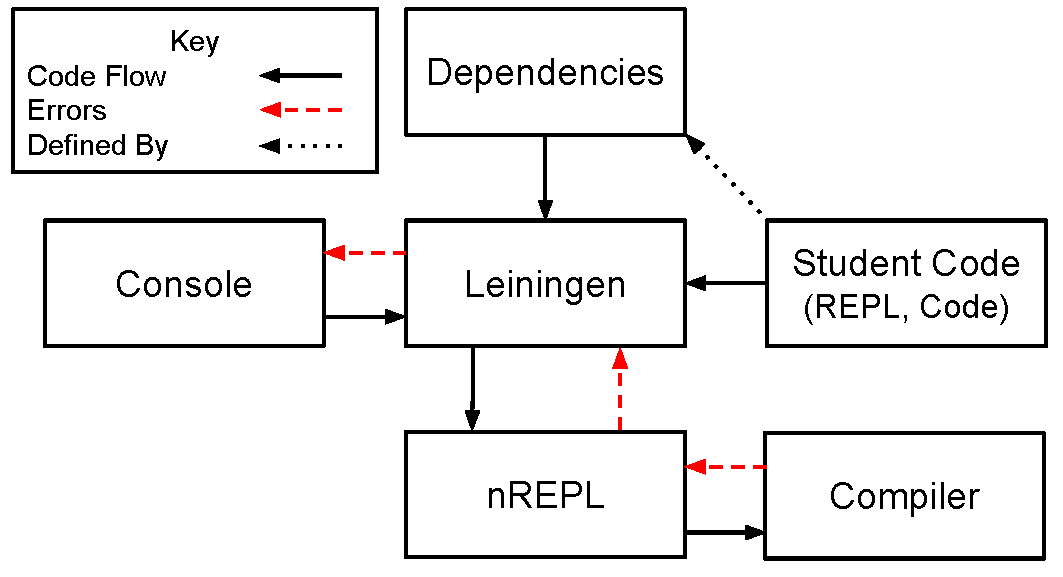
\includegraphics[width=10cm]{../CurrentErrorHandling.pdf}
 \centering
\end{figure}
\end{frame}

\begin{frame}
\frametitle{Issues 1}
	\begin{itemize}
		\item installation of Leiningen is nontrivial
		\item command line acts as a barrier
		\item we do not want students managing dependencies
		\item no integration with new error handling system
	\end{itemize} 
\end{frame}

\begin{frame}
\frametitle{Proposed Solutions}
	\begin{itemize}
		\item use scripting to abstract over Leiningen installation
		\item Graphical User Interface will abstract over command line
		\item Leiningen plugin to inject needed dependencies
		\item use nREPL to integrate new error handling system
	\end{itemize}
\end{frame}

\begin{frame}[fragile]
\frametitle{Proposed Workflow Diagram}
\begin{figure}[h]
 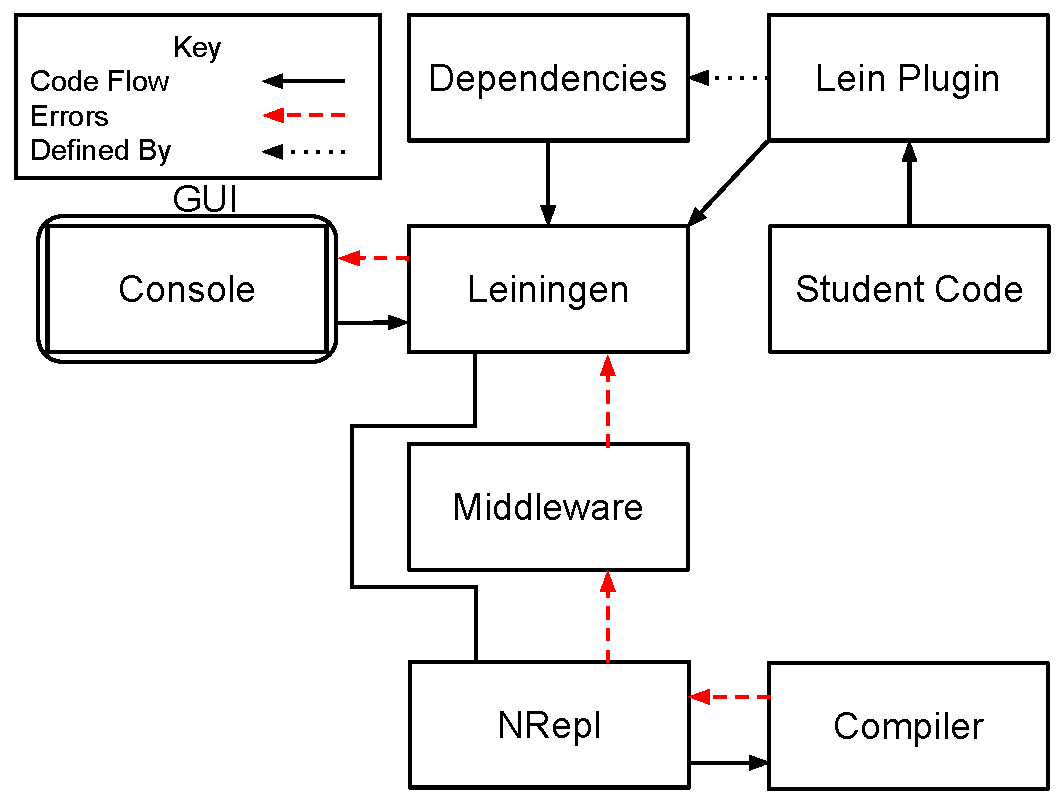
\includegraphics[width=9cm]{../OurErrorHandlingSystem.pdf}
 \centering
\end{figure}
\end{frame}

\begin{frame}
\frametitle{What needs to be done}
\end{frame}

\end{document}

